\documentclass[english]{article}
\usepackage[latin9]{inputenc}
\usepackage[letterpaper]{geometry}
\geometry{verbose,tmargin=1in,bmargin=1in,lmargin=1in,rmargin=1in}
\usepackage{amsmath}
\usepackage{amssymb}
\usepackage{graphicx}
\usepackage{float}
\usepackage{array}
\usepackage{tikz}
\usepackage{latexsym}
\usepackage{xspace}
\newcommand{\bx}{\mathbf{x}}
\newcommand{\bw}{\mathbf{w}}

\title{CIS 520, Machine Learning, Fall 2015: Assignment 5 \\
Due: Friday, October 23rd, 11:59pm}
\date{}
\author{Arpit Panwar}


\begin{document}
\maketitle
{\normalsize Collaborators: \\ 
\\ \underline{Sruthi Nair      }} \\

\section{Kernel Regression and Locally Weighted Regression}
\label{sec:regression}

Given a set of $n$ examples, $(\bx_i,y_i)$, $i=1,\ldots,n$, a linear
smoother is defined as follows. For any $\bx$, there exists a vector
$\ell(\bx)=(\ell_1(\bx),\ldots,\ell_n(\bx))^\top$ such that the
estimated output $\hat{y}$ of $\bx$ is
$\hat{y}=\sum_{i=1}^{n}\ell_i(\bx)y_i=\ell(\bx)^\top Y$ where $Y$ is a
$n\times 1$ vector, $Y_i=y_i$.  This means that the prediction is a
linear function of the training responses ($y_i$s) and it varies
slowly and smoothly with change or noise in $y_i$s.

\bigskip

\begin{enumerate}
\item (6 points) Recall that in linear regression with basis functions
  $h$, we assume the data are generated from the model
  $y_i=\sum_{j=1}^m w_j h_j(\bx_i)+\epsilon_i$. The least squares
  estimate for the coefficient vector $\bw$ is given by $\bw^*=(H^\top
  H)^{-1}H^\top Y$, where $H$ is a $n\times m$ matrix,
  $H_{ij}=h_j(\bx_i)$. Given an input $\bx$, what is the estimated
  output $\hat{y}$? (Matrix form solution is required. You may want to
  use the $m\times 1$ vector $h(\bx)=[h_1(\bx),\ldots,h_m(\bx)]^\top$)
  Is linear regression is a linear smoother? \\

Yes it is a linear smoother \\
\begin{align*}
	&\;\text{From the above we have}\\
	\hat{y} =&\; (w^{*}) h(x_i)^{\top} \\
	\text{Replacing the value of} w^{*} from \;above \\
	\hat{y} =&\; (H^\top  H)^{-1}H^\top Y h(x_i)^{\top}\\
	\text{Equating this with the equation for linear smoother we can say}\\
	\ell(x)^\top=&\;  (H^\top  H)^{-1}H^\top h(x_i)^{\top} \\
\end{align*}


\item (6 points) In kernel regression using the kernel $K(\bx_i,\bx)=
  \exp\{\frac{-||\bx_i-\bx||^2}{2\sigma^2}\}$, given an input $\bx$,
  what is the estimated output $\hat{y}$?  Is kernel regression is a
  linear smoother? \\
Yes it is a linear smoother \\
\begin{align*}
	&\;\text{We know that for kernel regression} \\
	\hat{y} =&\; \dfrac{ \sum\limits_{j=1}^n {K(x , x_j) y_j}}
			     {\sum\limits_{j=1}^n K(x , x_j)} \\
	&\;\text{Expanding the numerator} \\
	=&\; \dfrac{K(x,x_i)y_1 + K(x,x_2)y_2+K(x,x_3)y_3+ \ldots + K(x,x_n)y_n}
		        {\sum\limits_{j=1}^n K(x , x_j)} \\
	&\;\text{Splitting the above equation in terms of y vector} \\
	=&\; \left[    \dfrac{K(x,x_1)}{\sum\limits_{j=1}^n K(x , x_j)} , \ldots ,   \dfrac{K(x,x_n)}{\sum\limits_{j=1}^n K(x , x_j)}   \right ]
		\left[   \begin{array}{c}
				y_1\\
				y_2\\
				\ldots\\
				y_n
\end{array}	               \right] \\
	\ell(x_i) =&\; \left[    \dfrac{K(x,x_1)}{\sum\limits_{j=1}^n K(x , x_j)} , \ldots ,   \dfrac{K(x,x_n)}{\sum\limits_{j=1}^n K(x , x_j)}   \right ] \\
\end{align*}

\item (6 points) In locally weighted regression, given an input $\bx$,
  what is the estimated output $\hat{y}$?  Is locally weighted
  regression is a linear smoother? \\
The estimate is a linear smoother \\
\begin{align*}
	&\;\text{We know that for any x} x_k\\
	\hat{w}(x_k) =&\; argmin_w \sum\limits_{i=1}^n K(x_k,x_i) (w^\top x_i - y_i)^2 \\
	=&\; \frac{d}{dw} \sum\limits_{i=1}^n K(x_k,x_i) (w^\top x_i - y_i)^2 = 0 \\
	=&\;\sum\limits_{i=1}^n K(x_k,x_i) (w^\top x_i - y_i) 2x^\top = 0 \\
	0 =&\; \sum\limits_{i=1}^n K(x_k,x_i) w^\top x_i   2x^\top -  \sum\limits_{i=1}^n K(x_k,x_i) y_i 2x_i^\top \\
	&\;\text{solving for } w^\top \\
	w^\top =&\; \dfrac{\sum\limits_{i=1}^n K(x_k,x_i) y_i 2x_i^\top}
			     { \sum\limits_{i=1}^n K(x_k,x_i)  2x^\top x_i} = \hat{w}^{\top} \\
	&\;\text{We know } \hat{y}_k = \hat{w}(x_k)^\top x_k \\
	\hat{y}_k =&\; \dfrac{\sum\limits_{j=1}^n \sum\limits_{f = 1}^m  K(x_k,x_i) y_i 2x_{jf} x_{kf} }
				    {\sum\limits_{i=1}^n K(x_k,x_i)  2x^\top x_i  } \\ 
	\hat{y}_k =&\; \left[ \dfrac{\sum\limits_{f = 1}^m  K(x_k,x_1) 2x_{1f} x_{kf}} {\sum\limits_{i=1}^n K(x_k,x_i)   2x^\top x_i } \ldots   \dfrac{\sum\limits_{f = 1}^m  K(x_k,x_n) y_n 2x_{nf} x_{kf}} {\sum\limits_{i=1}^n K(x_k,x_i)   2x^\top x_i }           \right] \left[   \begin{array}{c}
				y_1\\
				y_2\\
				\ldots\\
				y_n
\end{array}	               \right] \\
	&\;\text{Equating it with the equation for } \hat{y} \text{ we get} \\
	l(x_k) =&\;  \left[ \dfrac{\sum\limits_{f = 1}^m  K(x_k,x_1) 2x_{1f} x_{kf}} {\sum\limits_{i=1}^n K(x_k,x_i)  2x^\top  x_i } \ldots   \dfrac{\sum\limits_{f = 1}^m  K(x_k,x_n) y_n 2x_{nf} x_{kf}} {\sum\limits_{i=1}^n K(x_k,x_i)  2x^\top x_i }           \right]&\; 
\end{align*}



\item (6 points) If we divide the range $(a,b)$ ($a$ and $b$ are real
  numbers, and $a<b$) into $m$ equally spaced bins denoted by
  $B_1,\ldots,B_k$.  Define the estimated output
  $\hat{y}=\frac{1}{|B_k|}\sum_{i:\bx_i\in B_k}y_i$, for $\bx\in B_k$,
  where $|B_k|$ is the number of points in $B_k$. In other words, the
  estimate $\hat{y}$ is a step function obtained by averaging the
  $y_i$s over each bin. This estimate is called the regressogram. Is
  this estimate a linear smoother? If yes, give the vector $\ell(\bx)$
  for a given input $\bx$; otherwise, state your reasons. \\
 The estimate is a linear smoother. \\
\begin{align*}
	\hat{y}=&\;\frac{1}{|B_k|}\sum_{i:\bx_i\in B_k}y_i \\ 
	&\;\text{By above, we know that the vector of weights will be 0 for all values except the bin the value is in} \\
	=&\; \left[ 0 \frac{1}{|B_1|} \ldots c \frac{1}{|B_i|} \ldots        \right]  \left[ 
					\begin{array}{c}
						y_1\\			y_2\\
						\ldots\\
						y_n
					\end{array}	       
        \right] \\
	&\;\text{Comparing it to the equation for linear smoother} \\
	\ell(x) =&\; \left[ 0 \frac{1}{|B_1|} \ldots c \frac{1}{|B_i|} \ldots  \right] \\
\end{align*}

\item (6 points) Suppose we fit a linear regression model, but instead
  of sum of residual squares $||H\bw-Y||_2^2$, we minimized the sum of
  absolute values of residuals: $||H\bw-Y||_1$. Is the result a linear
  smoother?  Prove (give formula for $\ell(\bx)$) or disprove (give a
  counter-example).  Hint: Think about the median---for a set of real
  numbers $(y_1,\ldots,y_n)$ where $n$ is odd, the median $y_M$
  minimizes the sum of absolute differences $M = \arg\min_j
  \sum_{i=1}^n |y_j - y_i|$. \\

It is not a linear smoother   \\

\begin{align*}
	&\; min_w (Hw - y) \\
	&\; min \left( \sum\limits_i h(x_i)^\top w - y_i \right) \\
	=&\; \frac{d}{dw} \sqrt{\left( \sum\limits_i h(x_i)^\top w - y_i \right) ^ 2} \\
	=&\; \sum\limits_i \frac{1}{2} \dfrac{2 (h(w_i)^\top w - y_i) h(x_i)^\top}
						     {\sqrt{(h(x_i)^\top w - y_i) ^ 2}} = 0\\
	=&\; \sum\limits_i \dfrac{(h(w_i)^\top w - y_i) h(x_i)^\top}
				       {|(h(x_i)^\top w - y_i)|} = 0\\
	&\;\text{We know that for a series of real numbers a median minimizes the series} \\
	&\;\text{We also know that for a linear series following must be true Median(A) + Median(B) = Median(A+B)} \\
	&\;\text {Whish can easily disproved by taking a simple 1-dimensional series}\\
	&\;\text{Thus we can say that the solution is non linear} \\
\end{align*}
  

\end{enumerate}
  
\section{Supervised Deep Learning}
\label{sec:sdl}

Neural networks are among the most powerful machine learning models, which can represent complex, non-linear functions. However, due to a high number of hyperparameters, neural networks are extremely difficult to tune for a particular task. In this exercise, we will apply neural networks for the task of handwritten digit recognition in a supervised and unsupervised setting. Specifically we will examine how the choice of different parameters affect the performance of a model. We provide all of the necessary code to complete this homework in \textit{DL\_toolbox} folder.


\bigskip

\begin{enumerate}
\item (5 points) File \textit{demo\_NN.m} contains the code required to train a neural network. You will now train two models: a plain neural network and a neural network that employs $L_2$ weight decay. Report the testing error of both models. Which model achieves lower testing error? Can you provide an explanation why? \\
Testing error for vanilla neural network = 0.0450 \\
Testing error with $L_2$ penalty = 0.0322 \\
The error is less when $L_2$ penalty is applied to the weights because when we penalize the weights we avoid overfitting. \\


\item (5 points) Now we will examine how a different choice of $L_2$ weight decay parameter affects the performance of the model. Use  \textit{demo\_NN\_L2\_decay.m} to train the models with $L_2$ weight decay parameters $0.01$ and $0.001$. Report the testing error achieved by both models. Which model performs better? How does the performance compare to the model that we trained in the previous part (ie. model that used $0.0001$ as its $L_2$ weight decay parameters)? Why? \\
For decay parameter $0.01$ the testing error = 0.1149 \\
For decay parameter $0.001$ the testing error = 0.0483 \\
The performance of the model is better when the error is $0.0001$ , the error increases when we increase the decay parameter because we don't train the model as well as we should when we add high penalties and as a result we underfit the test data. \\


\item (5 points) Dropout is a very popular technique in deep learning community that enforces regularization in the neural network. The basic idea behind dropout is simple: during the training a selected fraction of neurons are zeroed out. We will now explore how the choice of a dropout parameter affect the performance of the model. Use \textit{demo\_NN\_dropout.m} to train the model with dropout parameters of $0.25$ and $0.75$. That is, each of these models will zero out $25\%$ and $75\%$ of the neurons respectively. Report the testing error achieved by each of these models. Which parameter value achieves the best performance? Why? Does the dropout help to reduce testing error compared to the model without a dropout? \\
Test error when $0$ dropout = $0.0450$\\
Test error when $0.25$ dropout = $0.0421$\\
Test error when $0.75$ dropout = $0.0694$\\
The model with $25\%$ dropout gives the least test error but error increases when we increase the dropout as we begin to drop too many neurons and begin to underfit the test data. Additionally, Yes , the dropout helps reduce the test error as it avoids overfitting the training data. We can see that the error without dropout is higher as compared to error when dropout is $0.25$. \\

\item (5 points) Finally, we will examine how the size of a hidden layer affect the model's performance. Use \textit{demo\_NN\_hidden\_size.m} to train the model with hidden layer size parameters of $25, 100$ and $175$. Report the testing error achieved by each of these models. Which hidden layer size parameter achieves the best performance? Why do you think that is? Are there any disadvantages to the model that achieves lowest testing error relative to the model that achieves worst testing error in this case?\\
Error with Layer size $100$ = $0.0450$ \\
Error with layer size $25$ = $0.0602$ \\
Error with layer size $175$ = $0.0415$ \\
Error is minimized with layer size $175$ as it has more neurons and performs more regressions and thus produces a more accurate model. \\
The disadvantage of having $175$ neurons is it takes a long time to train the model and test it i.e. the process is very slow .\\

\end{enumerate}

\section{Unsupervised Deep Learning }
\label{sec:udl}

We now turn to unsupervised neural nets, which are also known as auto-encoders. Instead of minimizing the error with respect to ground truth, these models are trained to minimize the input reconstruction error (ie. treating input as ground truth). Auto-encoders can be viewed as models that learn a new non-linear feature representation. That is, we can take the hidden layers of a trained auto-encoder and use it as input features to a supervised learning method. In this exercise, we will examine if auto-encoders can learn a good feature representation and also how different parameter choices affect their performance.

\begin{enumerate}
\item (5 points) Use \textit{demo\_SAE.m} to train a plain auto-encoder. Visualize the learnt filters inside the auto-encoder using the \textit{visualize} function that is provided in the code. Embed the visualized filters in your writeup. Also save the trained model into \textit{models} directory as \textit{SAE.mat}. \\
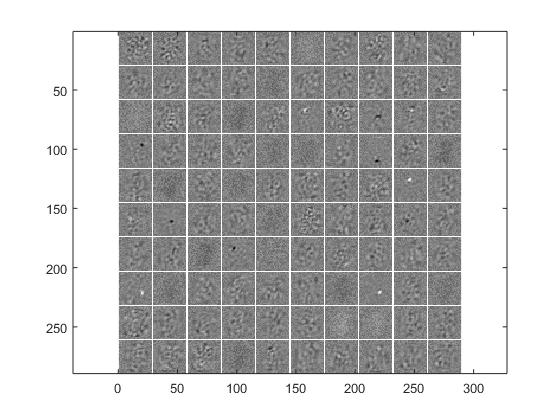
\includegraphics[width=90mm]{3_1.jpg} \\

\item (5 points) Use \textit{demo\_SAE.m} to train an auto-encoder with half of the input features zeroed out randomly. This parameter can be set by changing \textit{inputZeroMaskedFraction} parameter to $0.5$. Visualize the learnt filters inside the auto-encoder using the \textit{visualize} function that is provided in the code. Embed the visualized filters in your writeup. Also save the trained model into \textit{models} directory as \textit{SAE\_noisy.mat}. Visually compare the learnt filters from this part to the filters that were learnt in the previous part? What is the major difference? Judging from the visualizations do you think one of these auto-encoders learnt better features than the other? \\
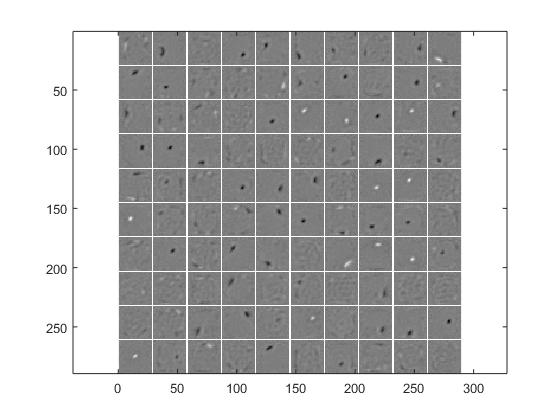
\includegraphics[width=90mm]{3_2.jpg} \\
The image in second part is sharper and has a lot clearer boundaries and features thus in second part the encoder learnt the features much better \\


\item (5 points) Take a look at \textit{demo\_SAE\_supervised.m} and use the hidden layer representation of autoencoder models from the previous parts as input to a supervised neural network. Do this with both models: \textit{SAE.mat} and \textit{SAE\_noisy.mat}. Report the testing errors achieved in both cases. Which auto-encoder features produce lower testing error? Does using the features learnt by auto-encoders achieves lower or higher testing error in comparison to using plain features? Compare the actual testing errors achieved by both approaches. \\
Testing error for noisy = $0.0285$ \\
Testing error for non-noisy = $0.0308$
Noisy gives lower error. \\
The error when learning auto-encoder is lower than when not learning using auto-encoder as learning using auto-encoder adds non-linear features as well to the model.\\


\end{enumerate}

\section{Lagrange Duality and the LASSO}
\label{sec:lag}

\begin{enumerate}
\item (5 points) The function \ref{Lasso21} is convex in $\mathbf{w}$ (quadratic plus $L_1$ norm), which means its minima satisfy $\nabla_w (\text{Eq.} \; \ref{Lasso21})=0$. Compute the gradient with respect to $\mathbf{w}$ of this expression and show that the resulting condition for any optimal $\mathbf{w}$ is
\begin{equation}\label{normalish}
\displaystyle \mathbf{0} = -\mathbf{X}^T(\mathbf{y}-\mathbf{X}\mathbf{w}) + \lambda \mathbf{v},
\end{equation}
where $\mathbf{v}=(v_1,\dots,v_m)\in\mathbb{R}^m$ satisfies
$v_i = 
\begin{cases} 
1 \quad \text{if} \quad w_i > 0\\
-1 \quad \text{if} \quad w_i < 0\\
\in[-1,1] \quad \text{if} \quad w_i = 0
\end{cases}$\\

\begin{align*}
	&\; \text{We know that the lagrange equation can be written as}\\
	L(w,\lambda) =&\; \frac{1}{2} \sum\limits_{i=1}^n \left( y_i - \sum_{j=1}^n x_{ij} w_j \right) ^2 + \lambda \sum_{j=1}^m |w_j| \\
	=&\; \frac{1}{2} (Y - Xw)^\top (Y - Xw) + \lambda \sum\limits_{j=1}^m |w_j| \\
	min_w L =&\; \frac{d}{dw} \frac{1}{2} (Y - Xw)^\top (Y - Xw) + \lambda \sum\limits_{j=1}^m |w_j| \\
	0 = &\; -X^\top (Y - Xw) + \lambda \sum\limits_{j=1}^m v_j \\
	0 = &\;  -X^\top (Y - Xw) + \lambda V \\
\end{align*}

\item (5 points) Set up the constrained optimization problem \ref{Lasso11} to be solved using the method of Lagrange multipliers. Write down the Lagrangian $L(\mathbf{w},\lambda)$ and Karush-Kuhn-Tucker conditions.\\
\begin{align*}
		L(w,\lambda) =&\; \frac{1}{2} \sum\limits_{i=1}^n \left( y_i - \sum_{j=1}^n x_{ij} w_j \right) ^2 + \lambda (\sum_{j=1}^m |w_j| -t) \\
		&\; \text{The KKT conditions are} \\
		i. \frac{d}{dw} L(w,\lambda) = 0\\
		ii. \lambda^* \ge 0 \\
		iii. \lambda^* (\sum_i |w_i| -t) = 0 \\
		iv. (\sum_i |w_i| -t) \le 0\\
\end{align*}

\item (5 points) Based on the discussion, we only need to find solutions for one case of the KKT conditions when $t<t_0$. Which case is this, and why?

\begin{align*}
	&\;\text{Based on the discussion we can formulate the following conditions} \\
	&\; t < t_0  \implies \lambda > 0 and \sum_j |w_j| = t \\
	&\; t \ge t_0 \implies \lambda = 0 \\
	&\;\text{Using these conditions we can say the following} \\
	&\;\text{Condition iii and iv are satisfied using eq 1} \\
	&\;\text{Condition ii is satisfied using eq 1 and 2} \\
	&\;\text{So all that's left is condition i which is } \frac{d}{dw} L(w,\lambda) = 0\\
\end{align*}

\item (5 points) Define\footnote{To be technical, this should be the supremum (least upper bound) rather than the maximum; we will not worry about this distinction here.}
\begin{equation}\label{primal}
\displaystyle L^*(\mathbf{w}) = \max_{\lambda \ge 0} L(\mathbf{w},\lambda)
\end{equation}
Show that 
\begin{equation}\label{primaleq}
L^*(\mathbf{w}) =\begin{cases} 
	f(\mathbf{w}) \quad \text{if} \quad (t - f_1(\mathbf{w})) \ge 0\\
	\infty \qquad \text{if} \quad (t - f_1(\mathbf{w})) < 0\\
\end{cases}
\end{equation}
	
Argue that, therefore, when $t<t_0$, minimizing $L^*(\mathbf{w})$ over all possible $\mathbf{w}$ is equivalent to solving the constrained optimization problem \ref{Lasso11}. Minimizing $L^*(\mathbf{w})$ is known as the \emph{primal problem}.\\
\emph{Hint: Show that if} $\mathbf{w}$ \emph{optimizes the constrained problem, then it also must minimize} $L^*$. \emph{Next, show that if} $\mathbf{w}$ \emph{minimizes} $L^*$, \emph{then it also must optimize the constrained problem. Proof by contradiction may be useful.}

\begin{align*}
		L(w,\lambda)^* =&\; max_{\lambda} \frac{1}{2} \sum\limits_{i=1}^n \left( y_i - \sum_{j=1}^n x_{ij} w_j \right) ^2 + \lambda \sum_{j=1}^m |w_j| -t \\
		=&\; \frac{d}{d\lambda} L = 0 \\
		=&\; \sum\limits_{j=1} |w_j| - t = 0 \\
		 \sum\limits_{j=1} =&\; t \\
		&\;\text{We can now see the equation}\\
		&\;when \; t - f_1(w) \ge 0 \text{ To maximize $L^*, \lambda$ will have to be 0} \\
		&\; and \;additionally \;when \; t - f_1(x) < 0 \; L^* will \; be \; maximized \; when \; \lambda = \infty\\
\end{align*}
Using above we can say that when w minimizes $L^*$ and thus it also minimizes $f(w)$. Additionally since $\sum |w_i| = t$ for t < $t_0$ , $L^* = f(w)$\\
Thus the w which minimizes $L^*$ will also minimize f(w)\\


\item (5 points) Define\footnote{Likewise, technically this should be the infimum (greatest lower bound) rather than the minimum.}
\begin{equation}\label{dual}
\displaystyle g (\lambda) =\min_{\mathbf{w} \in \mathbb{R}^m} L(\mathbf{w}, \lambda)
\end{equation}
Maximizing $g (\lambda)$ for $\lambda \ge 0$ is the \emph{dual problem} to the primal shown above.\\
	
One can show\footnote{since $L(\mathbf{w}, \lambda)$ is convex and goes to $+\infty$ as $||\mathbf{w}||_1\to\infty$} that, for fixed $\lambda$, $L(\mathbf{w},\lambda)$ has at least one minimum over $\mathbf{w}$. We can solve for a minimum in the usual way: by taking the gradient of $L$ with respect to $\mathbf{w}$ and setting it to zero. Do this to show that if $\bar{\mathbf{w}}$ minimizes $L(\mathbf{w}, \lambda)$ for fixed $\lambda$, then
\begin{equation}\label{normalish2}
\displaystyle \mathbf{0} = -\mathbf{X}^T(\mathbf{y}-\mathbf{X}\bar{\mathbf{w}}) + \lambda \mathbf{v},
\end{equation}
with $\mathbf{v}$ defined as before, in \ref{normalish}.\\

\begin{align*}
		L(w,\lambda)^* =&\; max_{\lambda} \frac{1}{2} \sum\limits_{i=1}^n \left( y_i - \sum_{j=1}^n x_{ij} \bar{w_j} \right) ^2 + \lambda \sum_{j=1}^m |\mathbf{w_j}| -t \\
		=&\; \frac{1}{2} (Y - Xw)^\top (Y - Xw) + \lambda \sum\limits_{j=1}^m |w_j| \\
		min_w L =&\; \frac{d}{dw} \frac{1}{2} (Y - Xw)^\top (Y - Xw) + \lambda \sum\limits_{j=1}^m |w_j| \\
		0 = &\; -X^\top (Y - X\bar{w}) + \lambda \sum\limits_{j=1}^m v_j \\
		0 = &\;  -X^\top (Y - X\bar{w}) + \lambda V \\
\end{align*}

\item (5 points) Show that $\mathbf{v}^T\bar{\mathbf{w}} = ||\bar{\mathbf{w}}||_1$. Consequently, show that if $\bar{\mathbf{w}}$ minimizes $L(\mathbf{w}, \lambda)$ for fixed $\lambda$, then 
\begin{equation}\label{wlambdarelation}
\lambda = (\mathbf{y}-\mathbf{X}\bar{\mathbf{w}})^T\mathbf{X}\bar{\mathbf{w}}/||\bar{\mathbf{w}}||_1.
\end{equation}\\

\begin{align*}
	\mathbf{v}^\top \bar{w} = \sum_{i} v_i * w_i \\
	\text{We know the values of v from problem 4.2} \\
	\mathbf{v} = ||\bar{w}||_1 \\
	\text{From the question 4.1 we can get $\lambda$ as} \\
	\lambda = \dfrac{X^\top (Y - Xw)}
			      {w}\\
	\lambda v = X^\top (Y - Xw) \\
	\text{Taking transpose} \\
	(\lambda v)^\top = (X^\top (Y - Xw)) ^\top \\
	\lambda v^\top = (Y - Xw)^\top X \\
	\lambda = \dfrac{ (Y - Xw)^\top X} {v^\top}\\
	\text{Replacing the value of $v^\top$}\\
	\lambda = (\mathbf{y}-\mathbf{X}\bar{\mathbf{w}})^T\mathbf{X}\bar{\mathbf{w}}/||\bar{\mathbf{w}}||_1
\end{align*}

\item (5 points) Matlab simulation for $t=6,10,14$...
	\begin{enumerate}
	\item For the different values of $t$, what do you notice about the differences between $\mathbf{w}_{MLE}$ (the solution computed for the OLS problem) and $\mathbf{w}_{OPT}$? How does the L1 penalty tend to zero out coefficients of $\mathbf{w}_{OPT}$ for the different values of $t$? Based on the coefficients used to generate the data (see in the file), is this what you'd expect?  \\
	
	$W_{MLE}$ is almost identical to $W_{OPT}$ when t = 14.  while the values when t=6 are greatly different.\\
	$L_1$ penalty for t = 6 is the highest and thus it zeroes out a lot of weights in $W_OPT$ \\
	Yes, since the variance of of $w_OPT$ when t=6 is 1 as the high penalty drives the weights to follow the variance of the disrtribution\\

	\item How do the computed $\lambda$'s change with $t$? Why is this? \\
	$\lambda$ is the highest when the error is the highest i.e. when t=6 and is lowest when the penalty is negligible i.e. t = 14\\	

	\end{enumerate}

\end{enumerate}

\end{document}
